\documentclass[a4paper,12pt]{article}

\usepackage{url}
\usepackage{epsfig}
\usepackage{graphics}
\usepackage{fancyhdr}

\graphicspath{{pictures/}}

\title{Carl Bildt Tweets: A comparison of regular and constrained Markov chain for text generation}
\author{\hspace*{-0.5cm}
Group Ain't intelligent\\
\begin{tabular}{cccc}
Viktor Bj\"{o}rkholm & Jesper Br\"{a}nn & Daniel Duberg & Jakob Tidestr\"{o}m\\
92-11-17 & 92-09-30 & 93-01-13 & 90-10-04 \\
viktorbj@kth.se & jbrann@kth.se & dduberg@kth.se & jakobti@kth.se \\
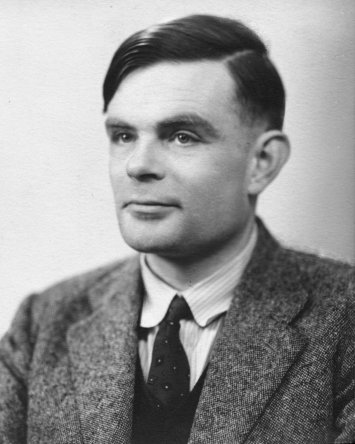
\includegraphics[width=0.13\linewidth]{Alan_Turing_photo} & 
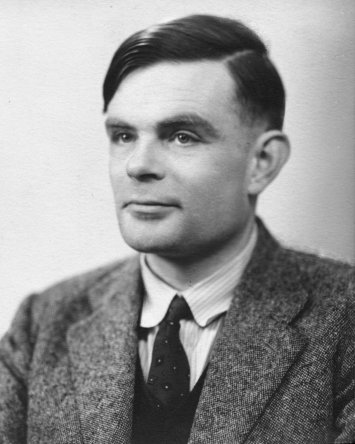
\includegraphics[width=0.13\linewidth]{Alan_Turing_photo} & 
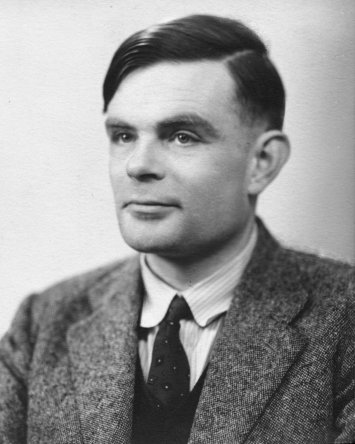
\includegraphics[width=0.13\linewidth]{Alan_Turing_photo} & 
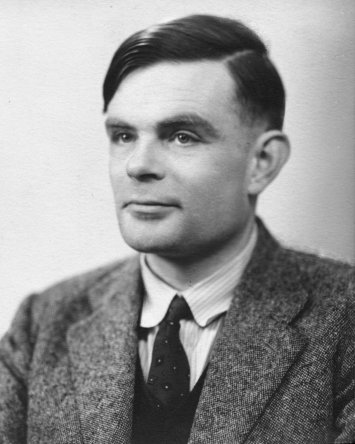
\includegraphics[width=0.13\linewidth]{Alan_Turing_photo}
\end{tabular}} 
% Normally there will not be any pictures but we want
% these so that we can connect faces to names in the course
% We also want birthdates so that we can tell people with the same
% name apart
\date{}

\pagestyle{fancy}
\setlength{\headheight}{15pt}
\fancyhf{}
\lhead{DD2380 ai14} % DO NOT REMOVE!!!!
\rhead{V. Bj\"{o}rkholm, J. Br\"{a}nn, D. Duberg, J. Tidestr\"{o}m} %% UPDATE WITH YOUR NAMES

\begin{document}

\maketitle
\thispagestyle{fancy}

\begin{abstract}
Skriv sist, när vi vet vad vi har skrivit om (y)
\end{abstract}



\clearpage

%%%%%%%%%%%%%%%%%%%%%%%%%%%%%%%%%%%%%%%%%%%%%%%%%%%%%%%%%%%%%
%%%%%%%%%%%%%%%%%%%%%%%%%%%%%%%%%%%%%%%%%%%%%%%%%%%%%%%%%%%%%
\section{Introduction (1--2 pages)}
\label{sec:intro}
There are a few approaches to generating text to make it seem like it was written by a human. One of these approaches is using Markov chains or more commonly known as n-grams. These n-grams take n words in sequence and uses a corpus of text to guess what the most probable next word is. Using a larger n means that more text is copied straight from the corpus, however this also means that there is a higher likelihood that the text being generated is meaningful.

In this paper we will generate twitter messages, tweets, using Markov chains. We explore the possiblity of using a unigram,  that is a 1-gram, with instead of words using parts-of-speeches to keep the grammatical structure of the corpus as well as keeping a \textbf{trigram} of words from the corpus to ensure that the semantical structure is also kept intact. This will be compared to the same model which is then constrained to a few predetermined criteria that we have selected, those being: The length and end state of the Markov chain. These criteria allows us to have a finer control over the Markov chain.

The concepts brought up in research by \cite{McBarb} are used and tweaked for our use case. Since twitter restricts messages to 140 characters we need to ensure that while generating messages long enough for the text to have a meaning, they should not go over the limit.


In this paper we compare the differences in result when using an n-gram on a corpus versus the result of using a constrained Markov model (uni- or bi-gram?). For the second implementation, basing our research on the work described in \cite{McBarb}, We opted for generating tweets with the same structure in the form of Parts-of-Words as our corpus dictated, in the second implementation basing our work on the research by .

-- Lite info om våra resultat --

   
\subsection{Contribution}
\textbf{Varfoer aer det vi gjort relevant?}

This paper contributes to the research field by 
Putting constraints on markov models seems to be a relatively recent approach. Our goal is to explore the \textbf{impact} of using constrained markov models to generate natural language.

\subsection{Outline}
Bla bla bla bla bla bla bla Section~\ref{sec:relwork} bla bla bla bla 
bla bla bla bla bla Section~\ref{sec:method} bla bla bla bla bla bla 
bla bla bla bla bla bla bla bla bla bla bla Section~\ref{sec:exps}
bla bla bla bla bla bla Section~\ref{sec:summary} bla bla bla bla bla

%%%%%%%%%%%%%%%%%%%%%%%%%%%%%%%%%%%%%%%%%%%%%%%%%%%%%%%%%%%%%
%%%%%%%%%%%%%%%%%%%%%%%%%%%%%%%%%%%%%%%%%%%%%%%%%%%%%%%%%%%%%
\section{Related work}
\label{sec:relwork}

Our work on the constrained Markov models are built upon \cite{McBarb} work, where the authors generated lyrics from different artists using Markov models with constraints. These were to be generated in a specific style and with a rhythm. However those criteria were not necessary for our work but we utilized the knowledge of constrained Markov models from them.



%%%%%%%%%%%%%%%%%%%%%%%%%%%%%%%%%%%%%%%%%%%%%%%%%%%%%%%%%%%%%
%%%%%%%%%%%%%%%%%%%%%%%%%%%%%%%%%%%%%%%%%%%%%%%%%%%%%%%%%%%%%
\section{My method}
\label{sec:method}



Our method consisted of building a transition matrix as a unigram of parts-of-speech (POS) together with a bigram with actual words from our corpus of text. From the transition matrix we generated a constrained transition matrix based on the amount of number of words we wanted the tweet to contain \textbf{(and other criteria)}. The constrained matrix was generated using the method described in the work by \cite{McBarb}. We generalized the method and made it work for our transition matrix even though it consisted only of parts-of-speech. 

The different constrains for creating a tweet that we had to consider were that they can not be longer than 140 characters, they have to end with an end-symbol (dot, exclamation mark or question mark) and they should probably have a reasonable minimum length. When iterating through a corpus we are using a POS-tagger to identify the different types of words and coding to be able to build a transition matrix for the sequences for the different word types (the probability for a noun to be followed by a word for an example). The next step is to implement our constraints on the transition matrix. The constraint for the length of the tweet caused us problems since we only know the types of the words and would not be in touch with the length of the specific words that are chosen for our tweet. We decided to approximate this constraint to a limited number of words in our tweet. 

\#yolo

\subsection{Implementation}
\label{sec:impl}
The implementation relied on a Part-of-Speech tagger from Stanford's Natural Language Processsing group.

%%%%%%%%%%%%%%%%%%%%%%%%%%%%%%%%%%%%%%%%%%%%%%%%%%%%%%%%%%%%%
%%%%%%%%%%%%%%%%%%%%%%%%%%%%%%%%%%%%%%%%%%%%%%%%%%%%%%%%%%%%%
\section{Experimental results}
\label{sec:exps}

Some images here and stuff would be nice.

\subsection{Experiemntal setup}
Bla bla bla bla bla bla bla bla bla bla bla bla bla bla bla bla bla 
bla bla bla bla bla bla bla bla bla bla bla bla bla bla bla bla bla 
bla bla bla bla bla bla bla bla bla bla bla bla bla bla bla bla bla 

\subsection{Experiment ...}

Bla bla bla bla bla bla bla bla bla bla bla bla bla bla bla bla bla 
bla bla bla bla bla bla bla bla bla bla bla bla bla bla bla bla bla 
bla bla bla bla bla bla bla bla bla bla bla bla bla bla bla bla bla 

\begin{figure}
\centering
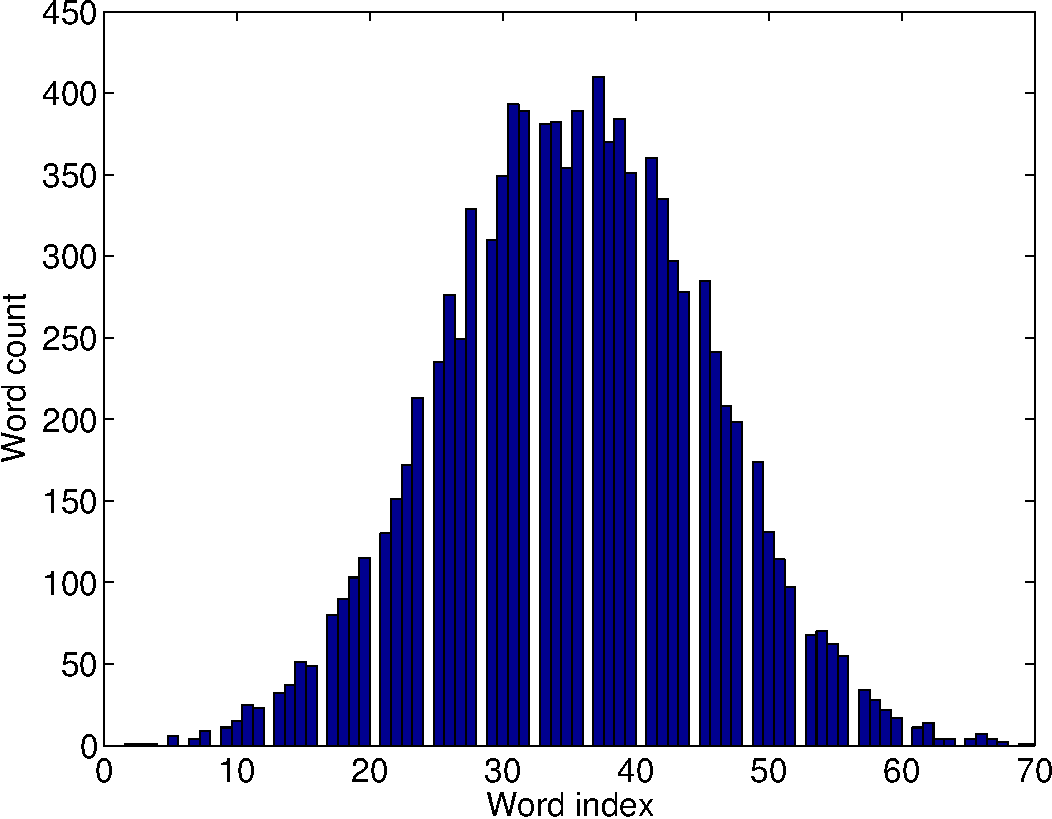
\includegraphics[width=0.8\linewidth]{histogram}
\caption{A description that makes browsing the paper easy and clearly 
describes what is in the picture. Make sure that the text in the figure 
is large enough to read and that the axes are labelled.}
\label{fig:histogram}
\end{figure}

Bla bla bla bla bla Figure~\ref{fig:histogram} bla bla bla bla bla bla 
bla bla bla bla bla bla bla bla bla bla bla bla bla bla bla bla bla 
bla bla bla bla bla bla bla bla bla bla bla bla bla bla bla bla bla 

\begin{table}
\begin{center}
\begin{tabular}{|c|c|c|}
\hline
Bla bla & Bla bla & Bla bla \\ \hline
42 & 42 & 42 \\ \hline
42 & 42 & 42 \\ \hline
\end{tabular}
\caption{A description that makes browsing the paper easy and clearly 
describes what is in the table.}
\label{tab:results}
\end{center}
\end{table}

Bla bla bla bla bla Table~\ref{tab:results} bla bla bla bla bla bla 
bla bla bla bla bla bla bla bla bla bla bla bla bla bla bla bla bla 
bla bla bla bla bla bla bla bla bla bla bla bla bla bla bla bla bla 

%%%%%%%%%%%%%%%%%%%%%%%%%%%%%%%%%%%%%%%%%%%%%%%%%%%%%%%%%%%%%
%%%%%%%%%%%%%%%%%%%%%%%%%%%%%%%%%%%%%%%%%%%%%%%%%%%%%%%%%%%%%
\section{Summary and Conclusions}
\label{sec:summary}

Bla bla bla bla bla bla bla bla bla bla bla bla bla bla bla bla bla 
bla bla bla bla bla bla bla bla bla bla bla bla bla bla bla bla bla 
bla bla bla bla bla bla bla bla bla bla bla bla bla bla bla bla bla 


%%%%%%%%%%%%%%%%%%%%%%%%%%%%%%%%%%%%%%%%%%%%%%%%%%%%%%%%%%%%%
%%%%%%%%%%%%%%%%%%%%%%%%%%%%%%%%%%%%%%%%%%%%%%%%%%%%%%%%%%%%%
\bibliographystyle{plain}
\bibliography{reflist}


\end{document}